%%%%%%%%%%%%%%%%%%%%%%%%%%%%%%%%%%%%%%%%%%%%%%%%%%%%%%%%%%%%%%%%%%%%%%%%%%%%%%%%%%%%%%%%%%%%%%%%
%
% CS484 Written Question Template
%
% Acknowledgements:
% The original code is written by Prof. James Tompkin (james_tompkin@brown.edu).
% The second version is revised by Prof. Min H. Kim (minhkim@kaist.ac.kr).
%
% This is a LaTeX document. LaTeX is a markup language for producing 
% documents. Your task is to fill out this document, then to compile 
% it into a PDF document. 
%
% 
% TO COMPILE:
% > pdflatex thisfile.tex
%
% If you do not have LaTeX and need a LaTeX distribution:
% - Personal laptops (all common OS): www.latex-project.org/get/
% - We recommend latex compiler miktex (https://miktex.org/) for windows,
%   macTex (http://www.tug.org/mactex/) for macOS users.
%   And TeXstudio(http://www.texstudio.org/) for latex editor.
%   You should install both compiler and editor for editing latex.
%   The another option is Overleaf (https://www.overleaf.com/) which is 
%   an online latex editor.
%
% If you need help with LaTeX, please come to office hours. 
% Or, there is plenty of help online:
% https://en.wikibooks.org/wiki/LaTeX
%
% Good luck!
% Min and the CS484 staff
%
%%%%%%%%%%%%%%%%%%%%%%%%%%%%%%%%%%%%%%%%%%%%%%%%%%%%%%%%%%%%%%%%%%%%%%%%%%%%%%%%%%%%%%%%%%%%%%%%
%
% How to include two graphics on the same line:
% 
% \includegraphics[width=0.49\linewidth]{yourgraphic1.png}
% \includegraphics[width=0.49\linewidth]{yourgraphic2.png}
%
% How to include equations:
%
% \begin{equation}
% y = mx+c
% \end{equation}
% 
%%%%%%%%%%%%%%%%%%%%%%%%%%%%%%%%%%%%%%%%%%%%%%%%%%%%%%%%%%%%%%%%%%%%%%%%%%%%%%%%%%%%%%%%%%%%%%%%

\documentclass[11pt]{article}

\usepackage[english]{babel}
\usepackage[utf8]{inputenc}
\usepackage[colorlinks = true,
            linkcolor = blue,
            urlcolor  = blue]{hyperref}
\usepackage[a4paper,margin=1.5in]{geometry}
\usepackage{stackengine,graphicx}
\usepackage{fancyhdr}
\setlength{\headheight}{15pt}
\usepackage{microtype}
\usepackage{times}
\usepackage{booktabs}

% From https://ctan.org/pkg/matlab-prettifier
\usepackage[numbered,framed]{matlab-prettifier}

\frenchspacing
\setlength{\parindent}{0cm} % Default is 15pt.
\setlength{\parskip}{0.3cm plus1mm minus1mm}

\pagestyle{fancy}
\fancyhf{}
\lhead{Homework Writeup}
\rhead{CS 484}
\rfoot{\thepage}

\date{}

\title{\vspace{-1cm}Homework 2 Writeup}


\begin{document}
\maketitle
\vspace{-3cm}
\thispagestyle{fancy}

\section*{Instructions}
\begin{itemize}
  \item Describe any interesting decisions you made to write your algorithm.
  \item Show and discuss the results of your algorithm.
  \item Feel free to include code snippets, images, and equations.
  \item Use as many pages as you need, but err on the short side If you feel you only need to write a short amount to meet the brief, th
  
  \item \textbf{Please make this document anonymous.}
\end{itemize}

\section*{In the beginning...}

I use fast Fourier transform convolution, by using 'fft' and 'ifft' functions in matlab. Fast Fourier transform (FFT) computes the discrete Fourier transform (or inverse) in O(NlogN). Definition of 1D-DFT is below.
\begin{figure}[h]
    \centering
    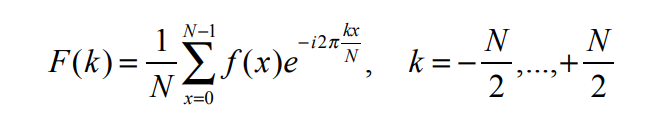
\includegraphics[width=7cm]{questions/DFT.PNG}
\end{figure}

\section*{Interesting Implementation Detail}



My code snippet (in 'my imfilter') highlights an interesting point.
\begin{lstlisting}[style=Matlab-editor]
for i=1:3
    '''implement the fft to A(padded image) and filter'''
    res{i} = ((sf-1)/2)+(1:sA);
    res2{i} = (sf-1)+(1:si);
end
'''implement convolution and ifft to A'''
A = A(res{:});
A = A(res2{:});
A = real(A);
output = A;
\end{lstlisting}
'Res' is intended to crop the image A after convolution, and res2 is intended to crop the cropped A in before-padded (original image) size.


\section*{A Result}

I use an example of 'mouse' which has 2 meanings, a computer input device and an animal.

\begin{figure}[h]
    \centering
    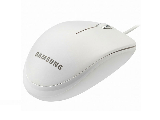
\includegraphics[width=5cm]{data/mouse2.png}
    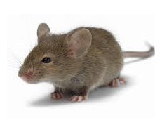
\includegraphics[width=5cm]{data/mouse1.png}
    \caption{\emph{Left:} computer input device 'mouse',  \emph{Right:} animal 'mouse'.}
\end{figure}

\begin{enumerate}
    \item Result 1 (Figure~\ref{fig:result1}, \ref{fig:result2}) was a failure, because cut-off frequency was too high, so the low frequencies image was too much blurred.
    \item Result 2 (Figure~\ref{fig:result3}, \ref{fig:result4}) was successful, because of the well-balanced cut-off frequency.
\end{enumerate}


\begin{figure}[h]
    \centering
    
\includegraphics[width=5cm]{questions/low_frequencies2.jpg}
    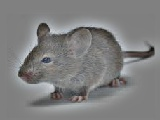
\includegraphics[width=5cm]{questions/high_frequencies2.jpg}
    \caption{\emph{Left:} low frequencies image,  \emph{Right:} high frequencies image.}
    \label{fig:result1}
\end{figure}

\begin{figure}[h]
    \centering
    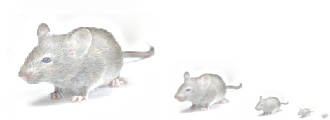
\includegraphics[width=10cm]{questions/hybrid_image_scales2.jpg}
    \caption{hybrid image (cut-off frequency is 7).}
    \label{fig:result2}
\end{figure}

\begin{figure}[h]
    \centering
    
\includegraphics[width=5cm]{questions/low_frequencies.jpg}
    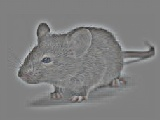
\includegraphics[width=5cm]{questions/high_frequencies.jpg}
    \caption{\emph{Left:} low frequencies image,  \emph{Right:} high frequencies image.}
    \label{fig:result3}
\end{figure}

\begin{figure}[h]
    \centering
    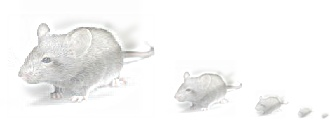
\includegraphics[width=10cm]{questions/hybrid_image_scales.jpg}
    \caption{hybrid image (cut-off frequency is 2.5).}
    \label{fig:result4}
\end{figure}
\begin{table}
    \centering
    \begin{tabular}{lrr}
        \toprule
         & Time (my imfilter) & Time (imfilter)\\
        \midrule
        Test 1 & 0.005113 & 0.001372\\
        Test 2 & 0.004367 & 0.000974\\
        Test 3 & 0.003161 & 0.001448\\
        \bottomrule
    \end{tabular}
    \caption{The efficiency of my code.}
    \label{tab:table1}
\end{table}

I compare the time taken to implement 'my imfilter' and 'imfilter'. My results are summarized in Table~\ref{tab:table1}. The results are surprising, because although my imfilter uses FFT, imfilter is faster than my imfilter. 

\end{document}
